\chapter{Introdução à análise ascendente}

\section{Introdução}

Até agora, estudamos técnicas \textbf{top-down} para a análise
sintática. Um analisador sintático top-down é limitado nas gramáticas
que pode processar, pois precisa ser capaz de decidir qual regra deve
ser usada com base em relativamente pouca informação. Por exemplo,
ele precisa ser capaz de escolher a produção correta a partir do
símbolo inicial com base no primeiro token da entrada.

Essa limitação motiva a análise sintática \textbf{bottom-up}, na qual
o analisador sintático pode escolher produções após analisar um
prefixo maior da entrada. Por exemplo, os analisadores sintáticos de
bottom-up podem lidar com produções recursivas à esquerda, enquanto
os analisadores sintáticos top-down não. De fato, os analisadores
sintáticos bottom-up funcionam melhor quando as produções são
recursivas à esquerda, embora também possam lidar com produções
recursivas à direita.

Neste capítulo, vamos apresentar dois algoritmos bottom-up: o
projetado por Earley e os algoritmos LR(0) e SLR.

\section{Algoritmo de Earley}

Um analisador sintático bottom-up expressivo e simples é o
desenvolvido por Jay Earley. Ele consegue analisar todas as
gramáticas livres de contexto, incluindo as ambíguas. Seu tempo de
execução no pior caso é cúbico em relação ao comprimento da entrada,
mas para a maioria das gramáticas encontradas na prática, leva tempo
linear se implementado com cuidado.

A ideia do analisador Earley é manter o controle de todas as análises
possíveis à medida que a entrada é lida. Podemos pensar no analisador
como aquele que, diferentemente de um analisador LL, não tenta prever
apenas uma produção; em vez disso, ele prevê cegamente todas as
possíveis produções, independentemente da decisão anterior, criando
uma nova thread concorrente para lidar com cada possível decisão. Um
problema dessa abordagem baseada em threads é o número exponencial de
threads criadas. Além disso, uma enorme quantidade de passos seria
repetido por diferentes threads. Portanto, o analisador Earley simula
o trabalho que essas threads fariam, garantindo que o trabalho seja
feito apenas uma vez.

O analisador Earley processa um token da entrada por vez, mantendo o
controle de todas as informações necessárias para simular as threads
de análise. Para cada posição de entrada \(j\), um analisador Earley
constrói um conjunto de itens \(I_j\) representando o estado das
produções que podem ser usadas na derivação. Um item Earley tem a
forma \([A \to \beta .\gamma, k]\). A primeira parte do item é uma
produção \(A \to \beta \gamma\) da gramática, com um ponto localizado
em algum lugar à direita da produção para indicar quanto dessa regra
de produção foi concluído. Para uma produção com o lado direito
vazio, como \(X \to \lambda\), a primeira parte do item contém apenas
o ponto: \([X \to ., k]\). A segunda parte do item, \(k\), é a posição
na entrada onde a análise do não-terminal $X$ começou, em termos do
número de tokens lidos até aquele ponto. Podemos pensar em \(k\) como
o registro da posição onde a thread para este item foi iniciada.

O algoritmo começa inicializando o conjunto \(I_0\) como \([S' \to .
S, 0]\), onde \(S\) é o símbolo inicial da gramática e \(S'\)) é um
novo símbolo de partida introduzido para simplificar o algoritmo. O
algoritmo analisa com sucesso a sequência de \(n\) tokens de entrada
\(a_0 a_1 ... a_{n - 1}\) se o item \([S' \to S ., 0]\) estiver no
conjunto \(I_n\).

O algoritmo considera cada posição de entrada \(j\) de 0 até n.~Em
cada posição de entrada, ele constrói o conjunto \(I_j\) aplicando as
três regras a seguir quantas vezes forem necessárias até que nenhuma
delas tenha efeito:

\begin{itemize}
\item \textbf{Verificar}. Se o conjunto \(I_j\) contém um item \([A \to
  \beta . c\delta, k]\) onde \(c\) é igual ao próximo símbolo de
  entrada \(a_j\), então o item \([A \to \beta c . \delta, k]\) é
  adicionado a \(I_{j+1}\). Todas as etapas de verificação podem ser
  realizadas como as ações finais em uma determinada posição de
  entrada, já que não afetam \(I_j\).
\item \textbf{Predição}. Se o conjunto \(I_j\) contém um item \([A \to
  \beta . C\delta, k]\), então, para todas as produções \(C\to
  \gamma\) na gramática, um item \([C\to.\gamma, j]\) é adicionado a
  \(I_j\). Observe que as etapas de predição podem habilitar etapas
  de predição adicionais, quando \(\gamma\) começa com um não terminal.
\item \textbf{Completar}. Se o conjunto \(I_j\) contém um item completo
  \([C\to \gamma . , k]\), então para cada item da forma \([A\to\beta
  . C\delta, l]\) no conjunto \(I_k\), um item \([A\to \beta C .
  \delta, l]\) é adicionado a \(I_j\).
\end{itemize}

Essas são as mesmas três ações que vimos no analisador LL baseado em
tabelas, mas, diferentemente daquele analisador, o analisador Earley
não precisa se compromenter com suas decisões. Em vez disso, ele lida
com múltiplas decisões, e até mesmo conclusões, em paralelo. As
previsões que não se confirmam são efetivamente descartadas, pois em
algum momento levam a itens incompatíveis com os tokens de entrada encontrados.

\subsection{Exemplo}

Considere a seguinte gramática, que não é LL(1):

\[
\begin{array}{lcl}
  S & \to & S\,+\,E\,\mid\,E\\
  E & \to & (\,E\,)\,\mid\,n\\
\end{array}
\]

Dado a entrada \verb|(1) + 2|, o analisador Earley
procede da seguinte forma:

\begin{table}[H]
\begin{tabular}{@{}lllll@{}}
  \toprule
  Conjunto & Item & Pos & Motivo & Etapa \# \\
  \midrule
  I0 & S' $\to$ . S & 0 & item inicial & 1 \\
  & S $\to$ . S + E & 0 & prever S & 2 (a partir de 1) \\
  & S $\to$ . E & 0 & prever S & 3 (a partir de 1 e também de 2) \\
  & E $\to$ . n & 0 & prever E & 4 (a partir de 3) \\
  & E $\to$ . ( S ) & 0 & prever E & 5 (de 3) \\
  \midrule
  I1 & E $\to$ ( . S ) & 0 & examinar ( & 6 (de 5) \\
    & S $\to$ . S + E & 1 & prever S & 7 (de 6) \\
    & S $\to$ . E & 1 & prever S & 8 (de 6 e também de 7) \\
    & E $\to$ . n & 1 & prever E & 9 (de 8) \\
    & E $\to$ . ( S ) & 1 & prever E & 10 (de 8) \\
    \midrule
    I2 & E $\to$ n . & 1 & consumir 1 & 11 (de 9) \\
    & S $\to$ E . & 1 & completar E & 12 (de 11, 8) \\
    & E $\to$ ( S . ) & 0 & completar S & 13 (de 12, 6) \\
    & S $\to$ S . + E & 1 & completar S & 14 (de 12, 7) \\
    \midrule
  I3 & E $\to$ ( S ) . & 0 & consumir ) & 15 (de 13) \\
  & S $\to$ E . & 0 & completo E & 16 (de 15, 3) \\
  & S' $\to$ S . & 0 & completo S & 17 (de 16, 1) \\
  & S $\to$ S . + E & 0 & completo S & 18 (de 16, 2) \\
  \midrule
  I4 & S $\to$ S + . E & 0 & consumir + & 19 (de 18) \\
  & E $\to$ . n & 4 & prever E & 20 (de 19) \\
  & E $\to$ . ( S ) & 4 & prever E & 21 (de 19) \\
  \midrule
  I5 & E $\to$ n . & 4 & consumir 2 & 22 (de 20) \\
  & S $\to$ S + E . & 0 & completo E & 23 (de 22, 19) \\
  & S' $\to$ S . & 0 & completo S: sucesso! & 24 (de 23, 1) \\
  & S $\to$ S . + E & 0 & completo S & 25 (de 23, 2) \\
  \bottomrule
\end{tabular}
\centering
\end{table}

Podemos visualizar a ação do analisador sintático desenhando um
gráfico que mostre como as várias etapas dependem umas das outras:

\begin{figure}[H]
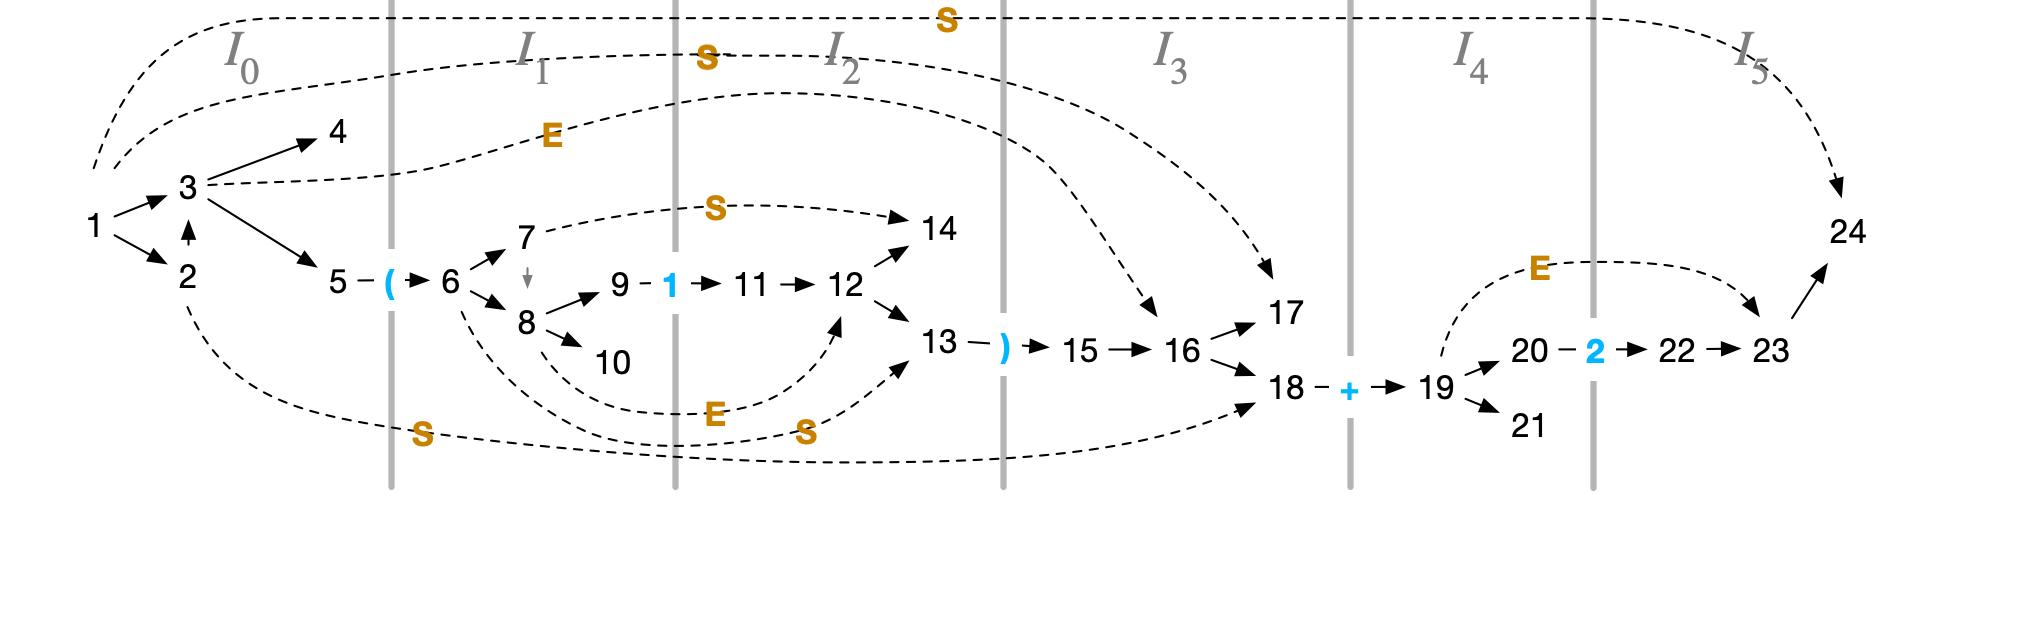
\includegraphics[scale=.4]{./chapters/earley-threads.png}
\centering
\end{figure}

Aqui, as ações de consumir tokens são anotadas com o token escaneado
em azul. As setas tracejadas mostram o estado e são rotuladas com o
não terminal que está sendo completado. Como este gráfico mostra, o
analisador explora alguns estados que não levam à análise
bem-sucedida, mas esses estados (4, 10, 14, 17 e 21) rapidamente
ficam \textbf{presos} porque não conseguem encontrar uma entrada
correspondente. Removendo esses estados e observando apenas a
sequência de produções completadas que levam ao sucesso na etapa 24,
vemos que elas descrevem uma derivação da string:

\[
\begin{array}{cccccccc}
  S' & \to & S & \to & S+E & \to & S+2 & \to \\
  24 &     & 23 &     & 18\text{--}22 &     & 16 &     \\[6pt]
  E+2 & \to & (S)+2 & \to & (E)+2 & \to & (1)+2 \\
  13\text{--}15 &     & 12 &     & 1\text{--}11 &     & \\
\end{array}
\]

Note que, a cada passo, o não terminal mais à direita é expandido
usando alguma produção. No entanto, o analisador sintático completa
essas produções de trás para frente, gerando a derivação mais à
direita invertida, começando pela entrada e terminando com o símbolo
inicial. Essa construção reversa de uma derivação mais à direita é o
que os analisadores sintáticos bottom-up fazem.

Os analisadores de Earley têm complexidade de tempo \(O(n^3)\) no
pior caso quando implementados cuidadosamente; em gramáticas não
ambíguas, a complexidade de tempo é \(O(n^2)\) no pior caso.
Intuitivamente, a razão pela qual os analisadores de Earley são
polinomiais em vez de exponenciais no pior caso é que eles
compartilham o trabalho entre as diferentes ``linhas de
processamento''. Por exemplo, observe que a conclusão única da
produção $S \to E.$ na etapa 12 realiza trabalho para duas linhas
de processamento que se ramificam na etapa 6 para os estados 7 e 8. A
linha de processamento ``7'' acaba ficando presa porque não encontra
o sinal ``+'' esperado na entrada, mas a outra linha de processamento
continua até o final.

Em gramáticas LL ou LR, os analisadores Earley são ainda mais úteis,
executando em tempo linear quando implementados cuidadosamente. Nossa
gramática de exemplo é uma gramática LR não ambígua, razão pela qual
o grafo de estados acima é predominantemente linear e pouco trabalho
é desperdiçado.

Uma otimização simples e útil é completar as produções somente quando
o token de lookahead estiver no conjunto FOLLOW do não terminal em
questão. Também pode ser útil memorizar etapas de predição em cascata.

Uma melhoria adicional que evita computação redundante é sugerida por
Aycock e Horspool
\href{https://academic.oup.com/comjnl/article-abstract/45/6/620/429185?redirectedFrom=PDF}{Practical
Earley Parsing}. Na etapa de predição, quando o símbolo C é anulável,
o item \([A\to \beta C.\gamma, k]\) é imediatamente adicionado ao
estado \(I_j\). Eles relatam que, com essa e outras otimizações, a
análise Earley é apenas 50\% mais lenta que o analisador LALR
Happy, uma compensação razoável dada a melhoria no poder de análise.

\section{Analisadores LR(0) e SLR}

A análise LR, incluindo a análise LALR, é um método popular de
análise sintática. Esses algoritmos são a tecnologia subjacente em
diversos geradores de analisadores sintáticos, como o Happy. Podemos
considerar a análise LR como uma otimização da análise Earley, na
qual todas as previsões são pré-computadas. A análise LR consiste em
duas ações: shift e reduce, portanto, os analisadores LR são chamados
de analisadores de shift-reduce. A ação de shift corresponde à ação
de consumo do algoritmo de Earley, seguida pelo máximo de previsões
possível; a ação de reduce corresponde à ação completa, novamente
seguida por previsões.

Em vez de manter o controle de todas as possíveis análises sintáticas
mais à direita, um analisador sintático de shift-reduce mantém o
controle apenas de um conjunto de análises sintáticas que
correspondem a uma única análise sintática mais à direita. Essa
limitação permite que o estado do analisador seja mais simples do que
em um analisador de Earley: o estado do analisador é baseado em uma
pilha de símbolos. Em qualquer ponto durante uma análise sintática de
shift-reduce, o estado atual da derivação é a concatenação da pilha
com a entrada não consumida. Por exemplo, podemos escrever a análise
sintática da expressão de exemplo \verb|(1)+2|
como uma série de operações de shift e reduce que constroem
exatamente a mesma derivação mais à direita que o analisador de
Earley fez acima:

\begin{table}[H]
\begin{tabular}{@{}lll@{}}
  \toprule
  Pilha de Derivação & Ações & Entrada não consumida \\
  \midrule
  (1) + 2 & (1) + 2 & \\
  (1) + 2 & shift & (1) + 2 \\
  (1) + 2 & shift & (1) + 2 \\
  (E) + 2 & reduce E $\to$ n & (E) + 2 \\
  (S) + 2 & reduce S $\to$ E & (S) + 2 \\
  (S) + 2 & shift & (S) + 2 \\
  E + 2 & reduce E $\to$ (S) & E + 2 \\
  S + 2 & reduce S $\to$ E & S + 2 \\
  S + 2 & shift & S + 2 \\
  S + 2 & shift & S + 2 \\
  S + E & reduce E $\to$ n & S + E \\
  S & reduce S $\to$ S+E & S \\
  \bottomrule
\end{tabular}
\centering
\end{table}

Para determinar qual ação deve ser tomada em cada etapa, o analisador
sintático precisa saber quais são as possíveis produções futuras a
serem reduzidas. As possíveis produções futuras são um conjunto de
itens, fechado sob predição; esse conjunto de itens nos diz qual ação
faz sentido em um determinado ponto da análise sintática. Para mapear
uma pilha em um conjunto de itens, esses conjuntos de itens podem ser
interpretados como um autômato finito determinístico que lê a pilha e
cujos estados são exatamente os conjuntos de itens. Esses estados são
semelhantes aos conjuntos de Earley, mas têm a propriedade de que,
ignorando a predição, apenas uma ação significativa pode ser tomada
em cada estado: shift ou reduce.

O estado inicial do autômato LR(0) corresponde ao conjunto de Earley
\(I_0\), exceto que adicionamos o símbolo de fim de entrada à
produção de nível superior. Assim como o conjunto de Earley, ele é
fechado sob predição.

\[
\begin{array}{l}
  S' \to . S \$\\
  S \to . S + E\\
  S \to . E\\
  E \to . n\\
  E \to . ( S )\\
\end{array}
\]

O autômato é construído repetindo-se o seguinte procedimento até que
nenhuma alteração adicional seja possível. Escolha um estado e um
símbolo que esteja à direita do ponto em uma ou mais produções.
Desloque esse símbolo para a direita nesses itens e feche o conjunto
de itens sob previsão. O conjunto de itens resultante pode ser um
estado existente do autômato ou um novo. Em ambos os casos, adicione
uma transição no símbolo escolhido do estado antigo para o estado
correspondente a este conjunto de itens.

\begin{figure}[H]
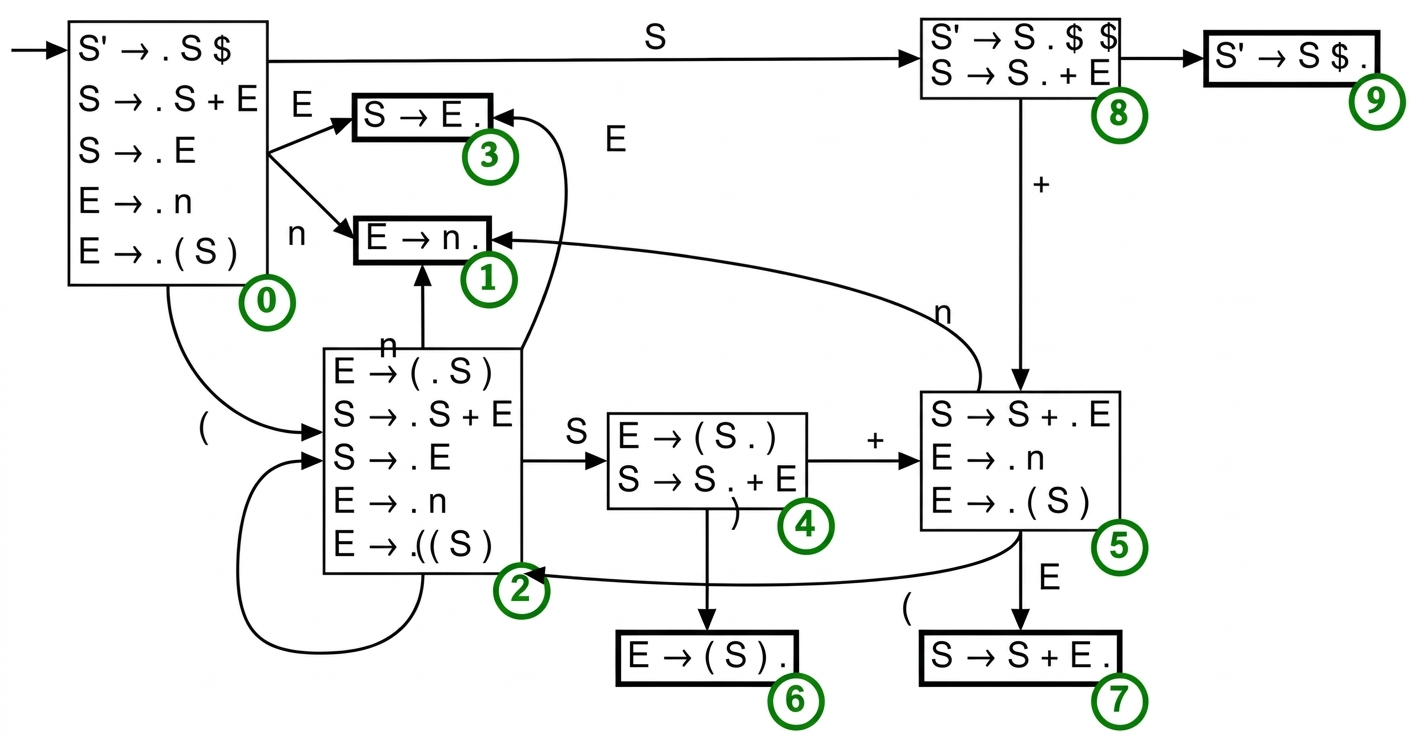
\includegraphics[scale=0.2]{./chapters/lr0.png}
\centering
\end{figure}

Por exemplo, ao realizar uma transição no token ( do estado inicial,
deslocamos apenas o último item para a direita, obtendo um estado
contendo a produção \(E \to ( . S )\), sobre o qual então realizamos
um fechamento de predição que adiciona itens para \(S\) e, em
seguida, para \(E\). Ao realizar uma transição a partir do mesmo
estado no não terminal S, deslocamos os dois primeiros itens para a
direita, obtendo os itens $S' \to S . \$$ e \(S \to S.+E\). O
fechamento de predição não adiciona nenhum item a este estado. A
figura a seguir mostra os passos que você pode seguir para completar
o autômato (pressione o botão para avançar a animação). Na figura, os
estados estão numerados em verde e os estados nos quais uma ação de
redução deve ser realizada têm uma borda mais espessa.

Podemos resumir este autômato em duas tabelas que podem ser usadas
para controlar um analisador sintático. A primeira é a tabela action,
que informa ao analisador o que fazer em cada estado, dado o símbolo
de previsão: shift e ir para um novo estado, ou reduce por alguma
produção. A segunda tabela é a tabela goto, que informa ao analisador
para qual estado ir quando ele reduz uma produção. Abaixo estão essas
duas tabelas do autômato que acabamos de construir, lado a lado.
Entradas vazias nas tabelas correspondem a erros de sintaxe. Entradas
numéricas na tabela action correspondem a ações de shift; uma
produção na tabela action indica uma ação de reduce.

\begin{table}[H]
  \begin{tabular}{@{}llllllll@{}}
    \toprule
    & n & + & ( & ) & \$ & S & E \\
    \midrule
    0 & 1 & & 2 & & & 8 & 3 \\
    1 & E $\to$ n & E $\to$ n & E $\to$ n & E $\to$ n & E $\to$ n & & \\
    2 & 1 & & 2 & & & 4 & 3 \\
    3 & S $\to$ E & S $\to$ E & S $\to$ E & S $\to$ E & S $\to$ E & & \\
    4 & & 5 & & 6 & & & \\
    5 & 1 & & 2 & & & & 7 \\
    6 & E $\to$ (S) & E $\to$ (S) & E $\to$ (S) & E $\to$ (S) & E
    $\to$ (S) & & \\
    7 & S $\to$ S+E & S $\to$ S+E & S $\to$ S+E & S $\to$ S+E & S
    $\to$ S+E & & \\
    8 & & 5 & & & 9 & & \\
    9 & \(S'\to S\). & \(S' \to S\). & \(S'\to S\). & \(S' \to S\). & \(S'\to
    S\$\). & & \\
    \bottomrule
  \end{tabular}
  \centering
\end{table}

Durante sua execução, um analisador sintático shift-reduce utiliza
uma tabela (como a apresentada) e uma pilha de estados. O algoritmo
inicia com a pilha contendo o estado inicial e a entrada a ser
processada. À medida que lê cada token de entrada, ele consulta na
tabela action qual é a ação atual para o estado no topo da pilha,
dado o próximo token. Se a ação for um shift, ele adiciona o estado
especificado à pilha. Se a ação for um reduce, ele remove da pilha o
número de itens na produção correspondente e usa a tabela goto do
estado agora no topo da pilha para determinar o próximo estado a ser
adicionado à pilha.

Vamos testar este analisador sintático no exemplo anterior,
\verb|(1)+2|. A pilha contém apenas o estado 0.
Para tornar mais claro, os estados na pilha são mostrados em
\textbf{negrito} e são precedidos pelo símbolo que foi seguido para
chegar a esse estado. Esses símbolos correspondem à parte da
derivação que foi construída até agora pelo analisador sintático.
\begin{table}[H]
  \begin{tabular}{@{}lll@{}}
    \toprule
    Pilha & Entrada & Ação \\
    \midrule
    \textbf{0} & (1)+2 & shift \textbf{2} \\
    \textbf{0}(\textbf{2} & 1)+2 & shift \textbf{1} \\
    \textbf{0}(\textbf{21} & )+2 & reduce E $\to$ n \\
    \textbf{0}(\textbf{2}E\textbf{3} & )+2 & reduce S $\to$ E \\
    \textbf{0}(\textbf{2}S\textbf{4} & )+2 & shift \textbf{6} \\
    \textbf{0}(\textbf{2}S\textbf{4})\textbf{6} & +2 & reduce E $\to$ (S) \\
    \textbf{0}E\textbf{3} & +2 & reduce S $\to$ E \\
    \textbf{0}S\textbf{8} & +2 & shift \textbf{5} \\
    \textbf{0}S\textbf{8}+\textbf{5} & 2 & shift \textbf{1} \\
    \textbf{0}S\textbf{8}+\textbf{51} & \$ & reduce E $\to$ n \\
    \textbf{0}S\textbf{8}+\textbf{5}E\textbf{7} & \$ & reduce S $\to$ S+E \\
    \textbf{0}S\textbf{8} & \$ & shift \textbf{9} \\
    \textbf{0}S\textbf{8}\$\textbf{9} & & reduce S' $\to$ S \\
    \bottomrule
  \end{tabular}
  \centering
\end{table}

Note que a construção LR que vimos até agora não faz nada além de
reduzir a uma única produção fixa, independentemente do próximo token
na entrada. Como resultado, os estados que contêm reduções (estados
1, 3, 6, 7, 9 no exemplo) ignoram o token de lookahead. A esse
algoritmo damos o nome de analisador LR(0). Preenchendo as tabelas de
action e goto de uma maneira menos restritiva, poderíamos obter um
analisador LR(1), que é mais expressivo. No entanto, precisaremos
modificar a construção da tabela LR(0) que acabamos de ver para obter
essa expressividade.

Uma extensão simples, mas surpreendentemente eficaz, para LR(0) é
adicionar uma ação de redução à tabela de ações apenas no caso em que
o token de lookahead esteja no conjunto FOLLOW do não terminal que
está sendo reduzido, já que, caso contrário, a produção claramente
não leva a uma análise válida. Quando esse refinamento na construção
LR(0) produz um analisador sintático shift-reduce válido, dizemos que
a gramática é SLR (Simple LR).

\section{Implementação}

Nesta seção comentamos os principais detalhes das implementações
Haskell dos algoritmos apresentados neste capítulo.

\subsection{Algoritmo de Earley}

A implementação está no módulo
\verb|Parsing.Earley.EarleyParser|. Os tipos
principais refletem diretamente as definições do algoritmo apresentadas acima.

\subsubsection{Itens e conjuntos}

Um item Earley \([A \to \beta . \gamma, k]\) é representado pelo tipo:

\begin{minted}{haskell}
data EarleyItem = EarleyItem
  { itemLhs :: String    -- não-terminal do lado esquerdo
  , itemBefore :: [Symbol]  -- símbolos antes do ponto
  , itemAfter :: [Symbol]  -- símbolos depois do ponto
  , itemOrigin :: Int -- posição de início
  }
\end{minted}

O campo \haskell{itemOrigin} corresponde ao índice
\(k\) do item \([A \to \beta.\gamma, k]\): ele registra em qual
conjunto Earley este item se originou, o que é usado na etapa de
completar. O chart completo é uma lista de conjuntos:

\begin{minted}{haskell}
type EarleySet = [EarleyItem]
type Chart = [EarleySet]
\end{minted}

O chart tem \(n + 1\) conjuntos, \(I_0\) a \(I_n\), onde \(n\) é o
comprimento da entrada.

\subsubsection{As três operações}

As três operações do algoritmo são funções puras:

\begin{minted}{haskell}
-- predição
predictItems :: Grammar -> Int -> EarleyItem -> [EarleyItem]
-- verificação
scanItems :: String -> EarleySet -> [EarleyItem]
-- completar
completeItems :: Chart -> EarleySet -> Int -> EarleyItem -> [EarleyItem]
\end{minted}

A função \haskell{completeItems} precisa de acesso ao
chart anterior para buscar os itens que esperavam o não-terminal
\(B\) completado. Quando o item completado tem
\haskell{itemOrigin = j < k}, a busca é feita em
\haskell{"chart !! j"} (já fechado); quando
\haskell{j = k}, busca-se em
\haskell{currentSet}, o conjunto sendo construído,
para lidar com completações em cadeia no mesmo conjunto.

\subsubsection{Fechamento de um conjunto}

A função \haskell{closeSet} aplica predição e
completar repetidamente usando um algoritmo de worklist: novos itens
gerados vão para o final da fila e são processados em ordem, evitando
elementos duplicados:

\begin{minted}{haskell}
closeSet :: Grammar -> Chart -> Int -> [EarleyItem] -> EarleySet
closeSet grammar prevSets k = go []
  where
    go current []           = current
    go current (item : rest)
      | item `elem` current = go current rest
      | otherwise =
          let current' = current ++ [item]
              new      = predictItems grammar k item
                      ++ completeItems prevSets current' k item
          in go current' (rest ++ new)
\end{minted}

Esta estrutura garante que cada item seja processado apenas uma vez,
assim como o algoritmo descrito na seção anterior assegura que as
três regras são aplicadas ``quantas vezes forem necessárias até que
nenhuma delas tenha efeito''.

\subsubsection{Construção do chart e aceitação}

A função \haskell{buildChart} constrói \(I_0\)
fechando os itens iniciais do símbolo de partida, depois aplica
\haskell{scanItems} para obter o conjunto inicial de
cada \(I_{k+1}\) e fecha-o:

\begin{minted}{haskell}
buildChart :: Grammar -> [String] -> Chart
buildChart grammar tokens = go [s0] tokens
  where
    s0 = closeSet grammar [] 0 startItems
    go chart []           = chart
    go chart (tok : toks) =
        let sk1 = closeSet grammar chart (length chart) (scanItems tok (last chart))
        in go (chart ++ [sk1]) toks
\end{minted}

A entrada é aceita se \(I_n\) contém um item completo para o símbolo
inicial com origem em 0, exatamente a condição \([S' \to S., 0]
\in I_n\) descrita na introdução do algoritmo:

\begin{minted}{haskell}
earleyParse :: Grammar -> [String] -> EarleyResult
earleyParse grammar tokens
    | any accept (chart !! n) = EarleyAccept
    | otherwise               = EarleyReject
  where
    n     = length tokens
    chart = buildChart grammar tokens
    accept item = itemLhs item == start && itemOrigin item == 0
               && null (itemAfter item)
\end{minted}

\subsection{LR(0) e SLR}

A implementação está distribuída em três módulos:
\begin{flushleft}
  \verb|Parsing.LR.LR0.BuildTable|,\\
  \verb|Parsing.LR.LR0.LR0Parser| e\\
  \verb|Parsing.LR.SLR.BuildTable|.
\end{flushleft}

\subsubsection{Itens e estados LR(0)}

Um item LR(0) \(A \to \alpha . \beta\) é mais simples que um item
Earley: não carrega a posição de origem, pois os estados do autômato
já capturam essa informação implicitamente:

\begin{minted}{haskell}
data Item = Item
  { itemLHS :: String    -- não-terminal
  , itemBefore :: [Symbol]  -- símbolos antes do ponto
  , itemAfter :: [Symbol]  -- símbolos depois do ponto
  }

type State = Set Item
\end{minted}

Um estado LR(0) é um conjunto de itens, exatamente como os conjuntos
de itens apresentados na seção anterior. O autômato cujos estados são
esses conjuntos é o DFA que lê a pilha do analisador.

\subsubsection{Fechamento e transições}

A função \haskell{closure} implementa o fechamento de
predição descrito no capítulo: para cada item com um não-terminal
\(C\) após o ponto, adiciona todos os itens \(C \to . \gamma\):

\begin{minted}{haskell}
closure :: Grammar -> State -> State
closure g = fixedPoint step
  where
    step current = Set.union current $ Set.fromList
        [ Item b [] prod
        | item <- Set.toList current
        , NonTerminal b <- take 1 (itemAfter item)
        , prod <- fromMaybe [] (Map.lookup b g)
        ]
\end{minted}

A função \haskell{goto} computa a transição do
autômato ao consumir um símbolo: avança o ponto nos itens que têm
esse símbolo imediatamente após ele e fecha o resultado:

\begin{minted}{haskell}
goto :: Grammar -> State -> Symbol -> State
goto g items sym = closure g $ Set.fromList
    [ Item lhs (before ++ [sym]) rest
    | Item lhs before (s:rest) <- Set.toList items
    , s == sym
    ]
\end{minted}

A função \haskell{buildStates} constrói a coleção
canônica de estados LR(0) por busca em largura, partindo do estado
inicial que contém o item \(S' \to . S\) da gramática aumentada:

\begin{minted}{haskell}
buildStates :: Grammar -> [State]
buildStates g = buildFrom [initial] [initial]
  where
    initial = closure g' (Set.singleton $ initialItem g')
    buildFrom seen [] = seen
    buildFrom seen (cur : queue) =
        let newStates = [goto g' cur sym | sym <- nextSymbols cur]
            unseen    = filter (`notElem` seen) newStates
        in buildFrom (seen ++ unseen) (queue ++ unseen)
\end{minted}

\subsubsection{Tabela de parsing LR(0)}

A tabela de parsing tem duas partes: a tabela
\haskell{action}, que mapeia
\haskell{(estado, terminal)} para uma ação, e a
tabela \haskell{goto}, que mapeia
\haskell{(estado, não-terminal)} para o próximo
estado após uma redução:

\begin{minted}{haskell}
data Action = Shift Int | Reduce String [Symbol] | Accept

data ParsingTable = ParsingTable
  { actionTable :: Map (Int, String) Action
  , gotoTable :: Map (Int, String) Int
  , states :: [State]
  }
\end{minted}

O preenchimento da tabela segue as regras descritas na seção de LR(0):

\begin{itemize}
  \item
    \textbf{Shift}: para cada terminal \(t\) após o ponto em algum
    item de um estado \(i\), action[i, t] = Shift j, onde
    \(j\) é o índice do estado
    \haskell{goto(i, t)}.
  \item
    \textbf{Reduce (LR(0))}: para cada item completo \(A \to \alpha
    .\) em um estado \(i\), action[i, t] =
    Reduce($A \to \alpha$) para \textbf{todos} os terminais \(t\) da
    gramática. Esta é a característica do LR(0): ele ignora o
    lookahead nas reduções.
  \item
    \textbf{Accept}: quando o item completo é \(S' \to S .\),
    action[i, \$] = Accept.
\end{itemize}

\subsubsection{O algoritmo de parsing LR(0)}

O algoritmo de parsing mantém uma pilha de estados e processa a
entrada símbolo a símbolo. O tipo
\haskell{ParserState} encapsula o estado completo do analisador:

\begin{minted}{haskell}
data ParserState = ParserState
  { stateStack :: [Int] -- pilha de estados
  , symbolStack :: [Symbol]  -- pilha de símbolos (para diagnóstico)
  , inputBuffer :: [String]  -- entrada restante
  }
\end{minted}

A função \haskell{parseStep} executa um único passo:
consulta action[estado\_topo, token] e
aplica a ação correspondente:

\begin{itemize}
  \item
    \textbf{Shift n}: empilha o estado \haskell{n} e
    avança na entrada.
  \item
    \textbf{Reduce $A \to \alpha$}: desempilha $\alpha$
    estados e empilha o estado dado por
    goto[novo\_topo, A]. Depois chama
    \haskell{parseStep} recursivamente pois a entrada
    não é consumida em reduções.
  \item
    \textbf{Accept}: sinaliza sucesso.
\end{itemize}

\begin{minted}{haskell}
parseLR0 :: Grammar -> ParsingTable -> [String] -> ParseResult
parseLR0 g table tokens = go (ParserState [0] [] (tokens ++ ["$"]))
\end{minted}

\subsubsection{A diferença do SLR}

O módulo \verb|Parsing.LR.SLR.BuildTable|
reutiliza toda a infraestrutura de LR(0):
\haskell{buildStates},
\haskell{closure}, \haskell{goto},
\haskell{parseLR0}. A implementação do SLR modifica apenas a geração
das entradas de redução. Enquanto LR(0) adiciona Reduce para todos os
terminais, SLR restringe às entradas cujo terminal pertence a
\(\mathrm{FOLLOW}(A)\):

\begin{minted}{haskell}
-- LR(0): reduz em todos os terminais
reduceA = [ ((i, t), Reduce lhs alpha)
          | item <- Set.toList state, null (itemAfter item)
          , t <- terminals g ++ ["$"] ]

-- SLR: reduz apenas nos terminais em FOLLOW(lhs)
reduceA = [ ((i, t), Reduce lhs alpha)
          | item <- Set.toList state, null (itemAfter item)
          , t <- fromMaybe [] (Map.lookup lhs followSets) ]
\end{minted}

Esta mudança pontual é suficiente para que a gramática de expressões
\[
  \begin{array}{lcl}
    E & \to  & E + T \\
    & \mid & T \\
    T & \to  & T * F \\
    & \mid & F \\
    F & \to  & (E) \\
    & \mid & n
  \end{array}
\]
deixe de ter conflitos: no estado que contém \(E \to T.\) e \(T
\to T.*F\), LR(0) colocaria Reduce \(E \to T\) em
$*$, gerando um conflito com Shift. Com SLR,
como \(* \notin \mathrm{FOLLOW}(E) = \{+, ), \$\}\), a entrada
action[estado, *] recebe apenas Shift, não resultando em conflito.

\section{Conclusão}

Este capítulo explorou técnicas bottom-up para análise sintática,
destacando como estas oferecem maior expressividade ao lidar com
recursão à esquerda e prefixos mais longos da entrada. Investigamos o
Algoritmo de Earley, uma solução robusta capaz de processar qualquer
gramática livre de contexto através da simulação de múltiplas frentes
de análise em paralelo, e introduzimos os fundamentos da análise
LR(0) e SLR, que otimizam esse processo via autômatos de shift-reduce
e pilhas de estados. Embora o SLR melhore a eficiência ao utilizar
conjuntos FOLLOW para decidir reduções, ele ainda apresenta
limitações em gramáticas mais complexas. Para superar essas
restrições, o próximo capítulo abordará os algoritmos LR(1) e LALR.
